\tikzset{every picture/.style={line width=0.75pt}} %set default line width to 0.75pt        

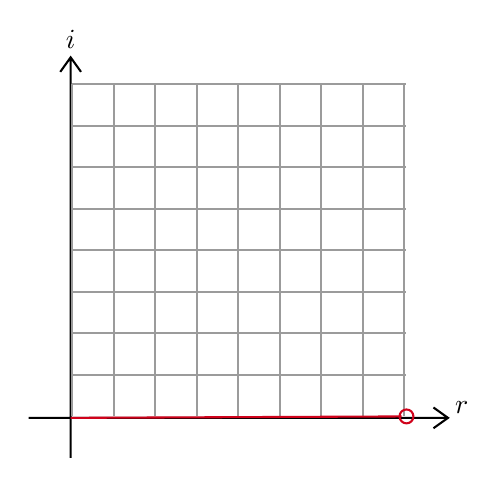
\begin{tikzpicture}[x=0.75pt,y=0.75pt,yscale=-1,xscale=1]
%uncomment if require: \path (0,300); %set diagram left start at 0, and has height of 300

%Shape: Axis 2D [id:dp5907524483347102] 
\draw  (267,209.7) -- (469,209.7)(287.2,36) -- (287.2,229) (462,204.7) -- (469,209.7) -- (462,214.7) (282.2,43) -- (287.2,36) -- (292.2,43)  ;
%Shape: Grid [id:dp6199898397920625] 
\draw  [draw opacity=0] (288,49) -- (449,49) -- (449,209) -- (288,209) -- cycle ; \draw  [color={rgb, 255:red, 155; green, 155; blue, 155 }  ,draw opacity=1 ] (288,49) -- (288,209)(308,49) -- (308,209)(328,49) -- (328,209)(348,49) -- (348,209)(368,49) -- (368,209)(388,49) -- (388,209)(408,49) -- (408,209)(428,49) -- (428,209)(448,49) -- (448,209) ; \draw  [color={rgb, 255:red, 155; green, 155; blue, 155 }  ,draw opacity=1 ] (288,49) -- (449,49)(288,69) -- (449,69)(288,89) -- (449,89)(288,109) -- (449,109)(288,129) -- (449,129)(288,149) -- (449,149)(288,169) -- (449,169)(288,189) -- (449,189) ; \draw  [color={rgb, 255:red, 155; green, 155; blue, 155 }  ,draw opacity=1 ]  ;
%Straight Lines [id:da9323494469903814] 
\draw [color={rgb, 255:red, 208; green, 2; blue, 27 }  ,draw opacity=1 ]   (287.2,209.7) -- (446.65,209.01) ;
\draw [shift={(449,209)}, rotate = 359.75] [color={rgb, 255:red, 208; green, 2; blue, 27 }  ,draw opacity=1 ][line width=0.75]      (0, 0) circle [x radius= 3.35, y radius= 3.35]   ;

% Text Node
\draw (287.23,33) node [anchor=south] [inner sep=0.75pt]    {$i$};
% Text Node
\draw (471,200.4) node [anchor=north west][inner sep=0.75pt]    {$r$};

\end{tikzpicture}
